The closed fuel cycle is one that includes the recycling of used, or spent, fuel
to be reused in a reactor. Spent fuel that exists the average Light Water
Reactor (LWR) has an elemental makeup shown in Table \ref{tab:lwr_fuel}. The
economics of recycling spent fuel is complicated and depends on many external
factors, but doing so has two overarching benefits that contribute to lowering
the cost of the fuel cycle: increasing repository capacity and increasing fuel
utilization. 

\begin{table} [h]
\centering
\begin{tabular} {|c|c|} 
\hline
Element Group & wt \% \\
\hline
Uranium           & $\mathrm{\sim}$95  \\
Plutonium         & $\mathrm{\sim}$1   \\
Mixed Actinides   & $\mathrm{\sim}$0.1 \\
Fission Products  & $\mathrm{\sim}$4   \\
\hline
\end{tabular}
\caption{Elemental Breakdown of Spent Fuel Exiting a Typical LWR}
\label{tab:lwr_fuel}
\end{table}

Of the elements that comprise used fuel, uranium, plutonium, and the mixed
actinides (MA) are all capable of producing power through the fission
process. The fission products, however, contain isotopes with high neutron
capture cross sections, which therefore act as poisons to the nuclear chain
reaction.  Achieving 100\% fuel utilization would thus require storing
indefinitely only the fission products and any other byproducts of the fuel
cycle. Furthermore, repository capacity is determined not necessarily by total
mass, but rather by heat load and radiotoxicity, making the concentration of
high-activity isotopes the limiting factor in a repository's capacity. Fission
products are generally short-lived (in comparison to transuranic elements, i.e.,
uranium, plutonium, and the MAs). Accordingly, by minimizing the amount of
transuranics in a repository, its capacity can be extended.

The act of reprocessing spent fuel is a requires relatively few steps. Once fuel
has left the reactor core, it is stored in a spent fuel pool for a some number
of years, typically around five. It can then be directly sent to a reprocessing
facility or be sent after some period of dry-cask storage. Reprocessing fuel is
a chemical extraction process and therefore is limited by chemical extraction
techniques. In general, there are two types of such processes: low-temperature
methods using organic solvents (e.g. PUREX), and high-temperature methods using
molten salts and metals, called pyroprocessing. The extraction techniques
separate the spent fuel into chemically-similar groups which can be different
based on the technique used. However, the separated groups are usually some
combination of those shown in Table \ref{tab:lwr_fuel}. The separated streams
are then sent either to a repository as high-level waste (HLW) or to an
appropriate fuel fabrication facility. Graphically, the closed fuel cycle is
shown in Figure \ref{fig:closed-cycle}.

\begin{figure}[]
  \begin{center}
    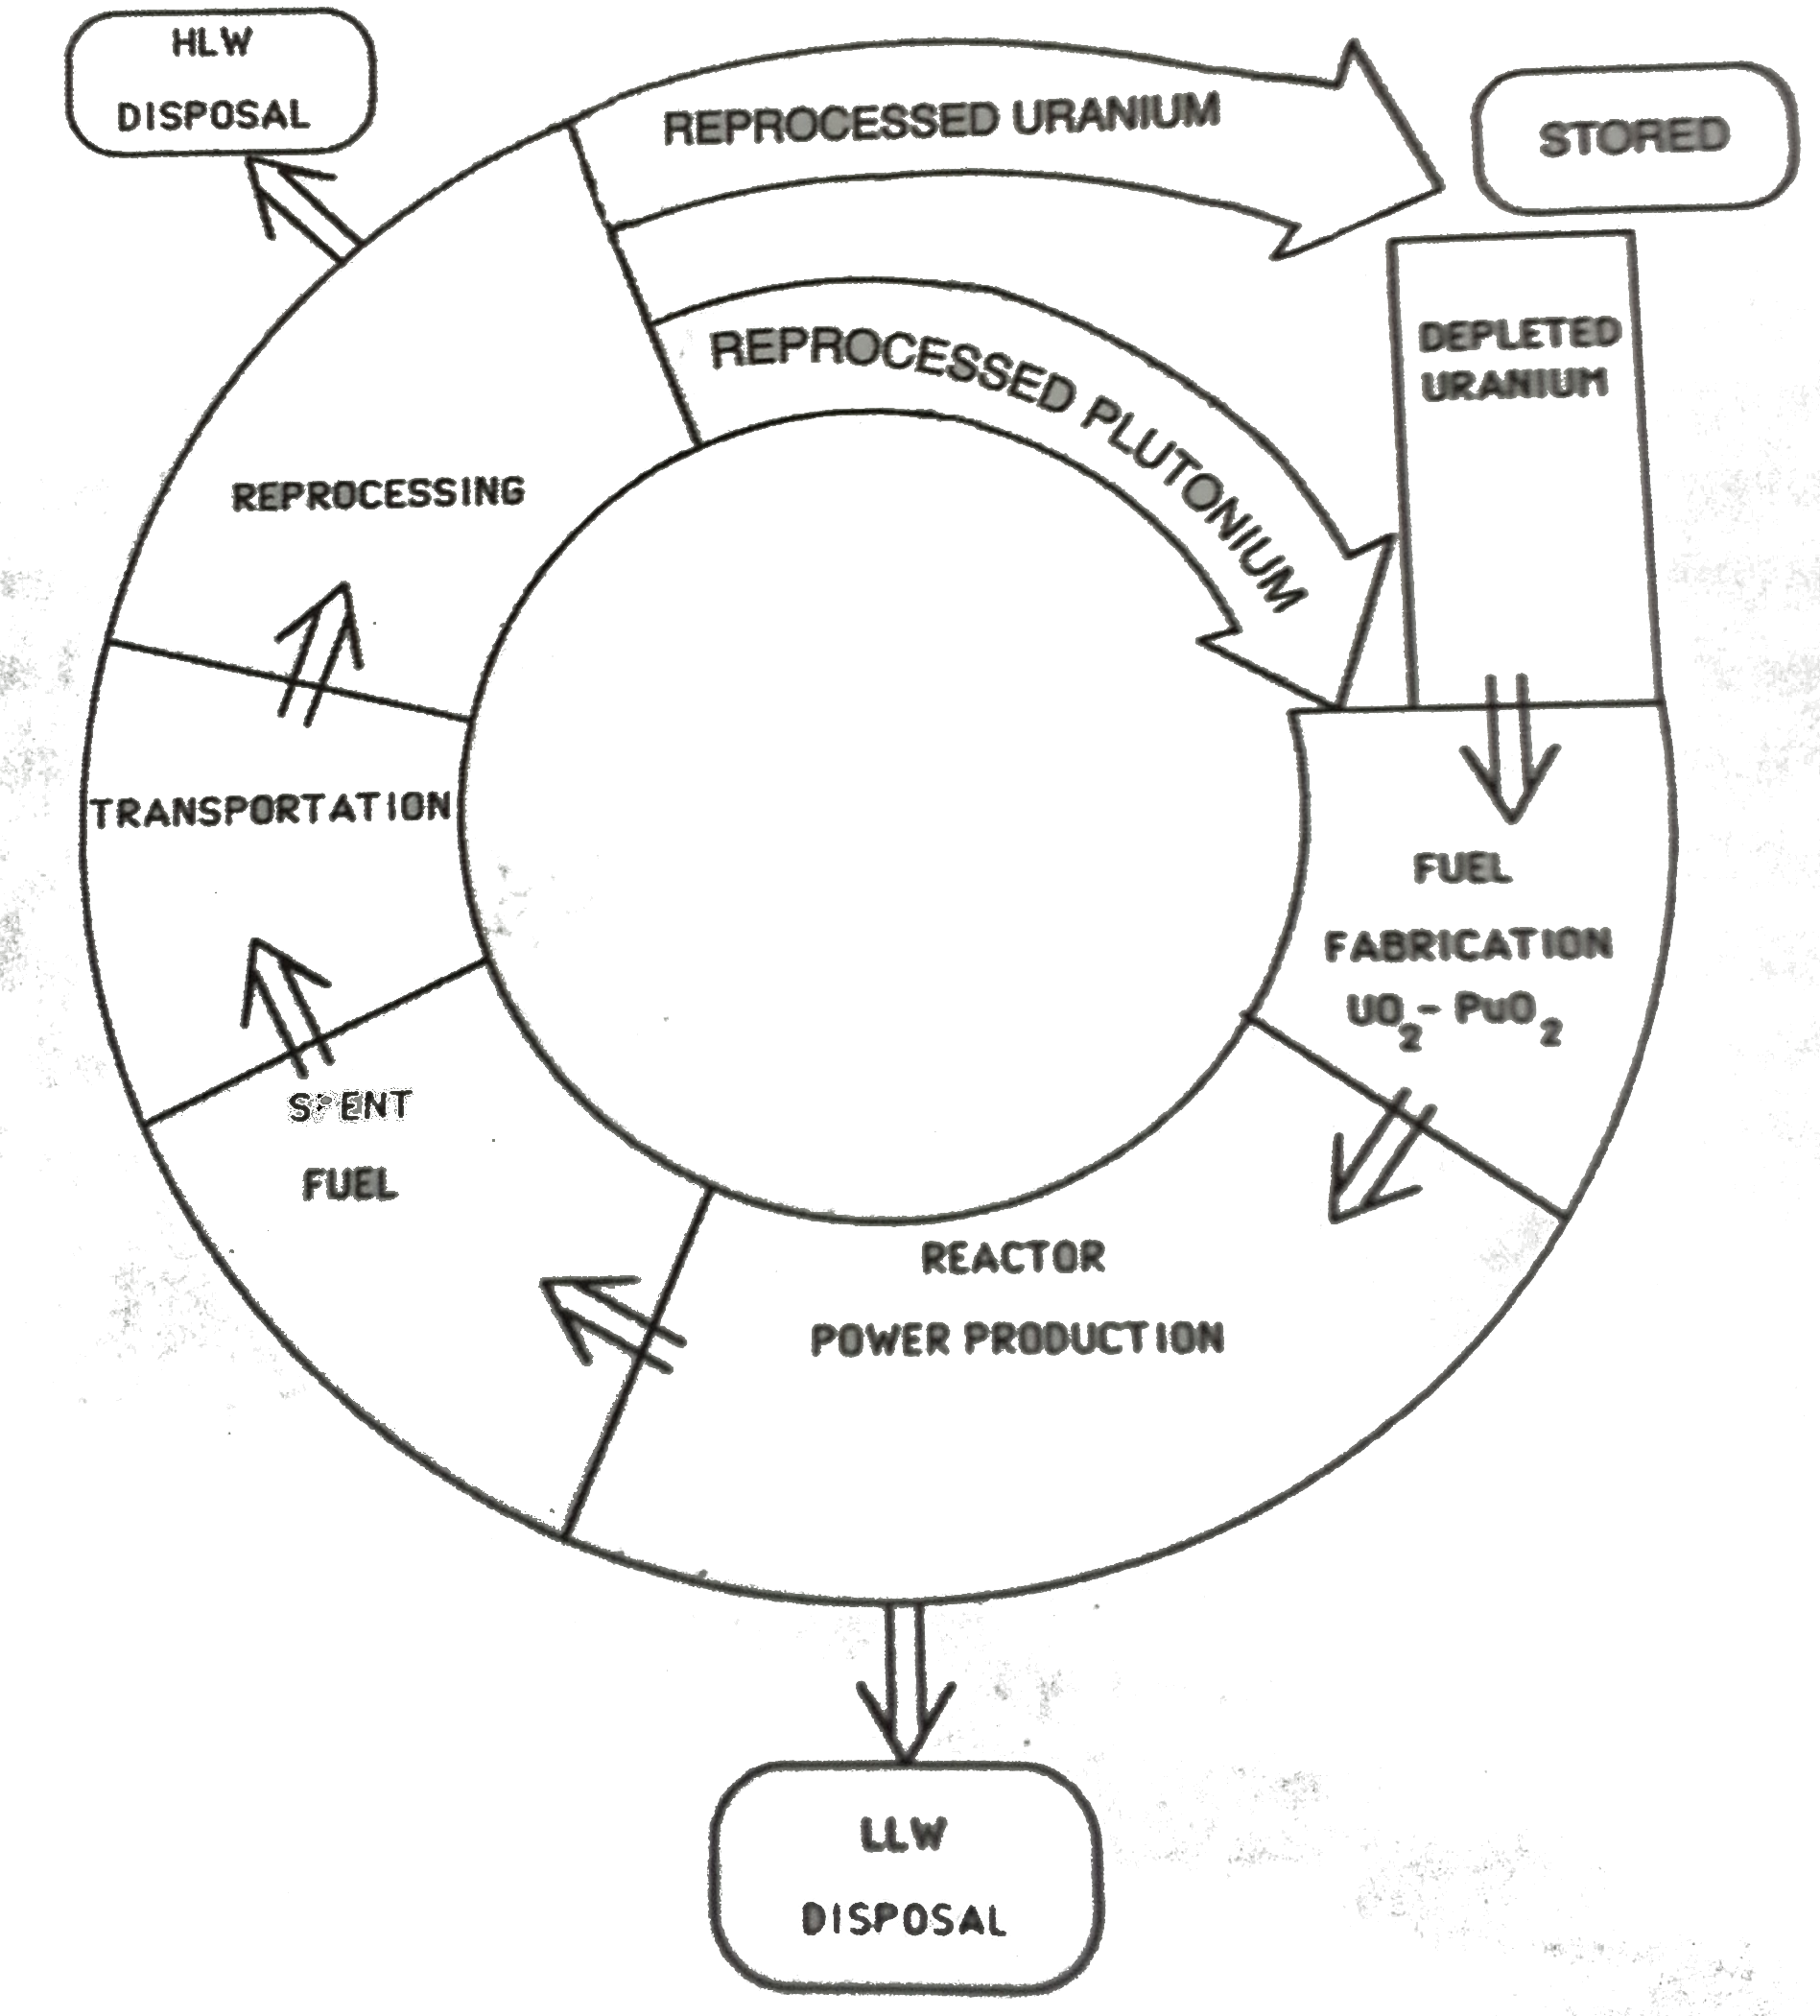
\includegraphics[height=7.5cm]{./chapters/intro/closed_cycle.png}
  \caption{The closed fuel cycle as shown in \cite{cochran1990nuclear}.}
  \label{fig:closed-cycle}
  \end{center}
\end{figure}


The elemental groups used in fuel fabrication will depend on the fuel cycle that
is developed. The only large-scale industrial reprocessing plants (La Hague in
France, THORP in the U.K., Mayak in Russia, and Rokkasho in Japan) utilize the
PUREX process to extract uranium and plutonium. The plutonium is then oxidized
and mixed with depleted Uranium from the enrichment process to produce what is
known as mixed-oxide fuel (MOX). Other sources of uranium can be used to fill
MOX fuel, as neutronics-related reactivity and safety constraints allow. Other
fuel cycles utilize the mixed actinides elemental group as well. These generally
include fast reactors that convert their transuranics inventory into either more
TRU (i.e., they have a conversion ratio (CR) of greater than 1), less TRU (CR <
1), or they maintain the amount of TRU entering and exiting their system (CR =
1). Fast reactors with CR > 1 are called breeder reactors.

It should be noted that with any reprocessing capability, nonproliferation
issues arise. Nuclear weapons have historically been produced using either
enriched uranium or plutonium; however it is possible to produce one with any
mix of appropriate materials. Accordingly, any fuel cycle that exposes bare
plutonium streams has an inherently higher nonproliferation risk than one that
does not, and such risks must be weighed accordingly. On a technical note,
though, the relatively low content of Pu-239, especially with respect to the
concentration of heat-producing Pu-240, in spent LWR fuel makes diverting such
fuel for the purposes of nuclear weaponry a route with a near-non-existant
probability of success.
